\documentclass[border=3pt]{standalone}
% Preâmbulo compartilhado pelos diagramas TikZ da aula 7 de IHC (Organização do Espaço de Problema)
\usepackage[T1]{fontenc}
\usepackage[utf8]{inputenc}
\usepackage{lmodern}
\usepackage{amsmath}
\usepackage{xcolor}
\usepackage{tikz}
\usetikzlibrary{arrows.meta,angles,quotes,decorations.pathmorphing,calc,
                positioning,shapes.geometric,shapes.misc,backgrounds,fit,
                math}

% Paleta (mesma dos SVGs originais)
% Paleta da disciplina de IHC: acento roxo (#755099), da capa do livro.
% (o nome "dblue" é mantido para não alterar todos os diagramas)
\definecolor{dblue}{HTML}{755099}
\definecolor{dorange}{HTML}{B3541E}
\definecolor{dgreen}{HTML}{4A7C59}
\definecolor{dred}{HTML}{9C4B4B}
\definecolor{dcream}{HTML}{F4F1EA}
\definecolor{dshade}{HTML}{DDD7C9}

% Função gaussiana (não normalizada por padrão de escala visual)
\pgfmathdeclarefunction{gauss}{3}{%
  \pgfmathparse{1/(#3*sqrt(2*pi))*exp(-((#1-#2)^2)/(2*#3^2))}%
}

% Estilos comuns (prefixo d... para não colidir com chaves internas do pgf)
\tikzset{
  >={Stealth[length=2mm]},
  dguide/.style={gray!55, dashed, line width=0.4pt},
  daxis/.style={gray!60, line width=0.7pt, ->},
  dbody/.style={fill=black!3, draw=black!80, line width=1pt},
  dacc/.style={draw=dblue, line width=1pt},
  dlbl/.style={black!55, font=\small},
  dsub/.style={black!45, font=\footnotesize},
  dstate/.style={circle, draw=black!80, fill=dcream, line width=1pt,
                 minimum size=17mm, font=\large, inner sep=1pt},
  dobs/.style={circle, draw=black!80, fill=dshade, line width=1pt,
               minimum size=14mm, font=\large, inner sep=1pt},
  dbox/.style={rounded corners=2pt, draw=black!80, fill=dcream, line width=1pt,
               align=center, inner sep=6pt},
  dop/.style={circle, draw=black!80, fill=white, line width=1pt,
              minimum size=6mm, inner sep=0pt, font=\small},
  dtrans/.style={->, dblue, line width=1pt},
  dmeas/.style={->, dorange, line width=1pt},
  dcurve/.style={line width=1pt, dblue},
  dcurveb/.style={line width=1.4pt, dorange},
}

\begin{document}
\hyphenpenalty=10000 \exhyphenpenalty=10000 \tolerance=9999 \emergencystretch=3em
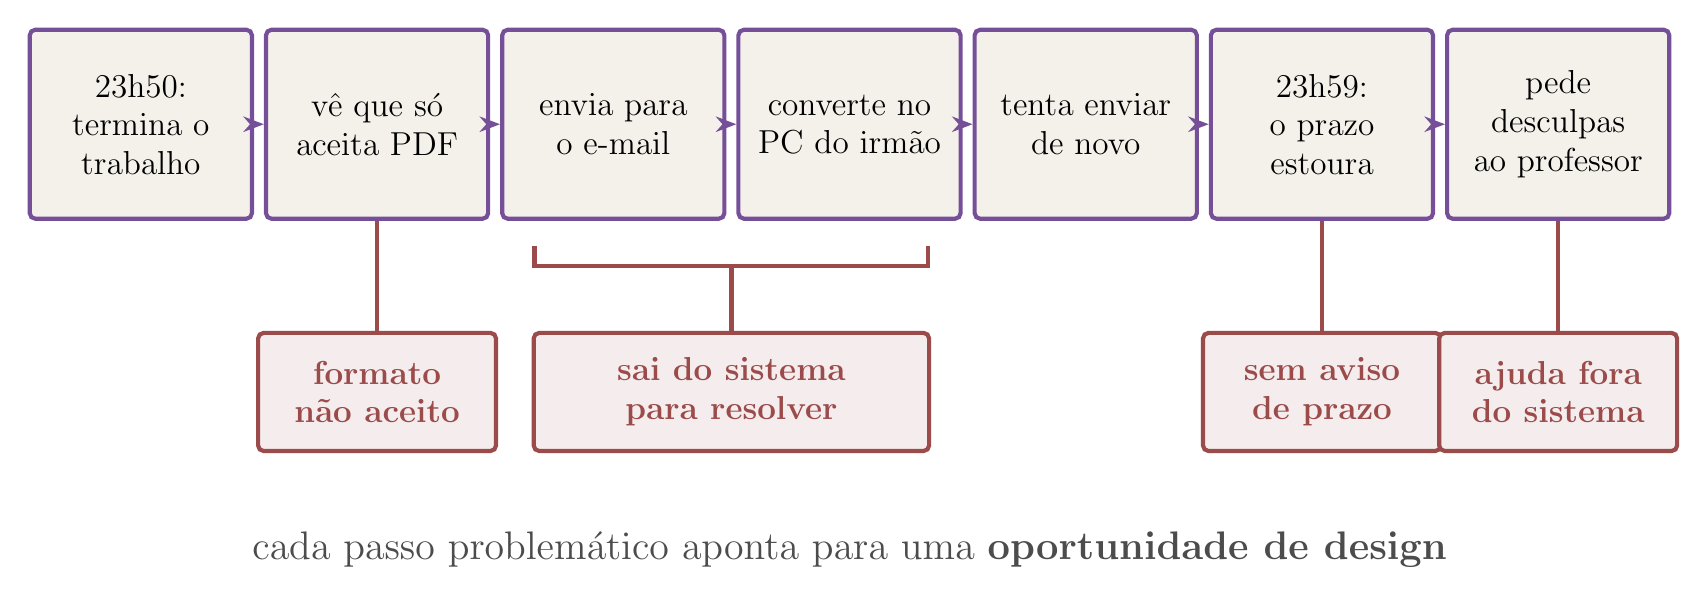
\begin{tikzpicture}[x=1cm,y=1cm]
  \tikzset{p/.style={dbox, draw=dblue, line width=1.5pt, text width=2.4cm, minimum height=2.4cm, font=\large}, r/.style={dbox, draw=dred, fill=dred!10, line width=1.5pt, font=\large\bfseries, text=dred, text width=2.6cm, minimum height=1.5cm}}
  \foreach \i/\t in {1/{23h50: termina o trabalho}, 2/{vê que só aceita PDF}, 3/{envia para o e-mail}, 4/{converte no PC do irmão}, 5/{tenta enviar de novo}, 6/{23h59: o prazo estoura}, 7/{pede desculpas ao professor}} {
    \node[p] (s\i) at (\i*3.0,0) {\t};
  }
  \foreach \i in {1,2,3,4,5,6} {
    \pgfmathtruncatemacro{\j}{\i+1}
    \draw[dtrans, line width=1.8pt, -{Stealth[length=2.6mm]}] (s\i.east) -- (s\j.west);
  }
  % problemas
  \node[r] (a) at (6.0,-3.4) {formato não aceito};
  \draw[dred, line width=1.6pt] (a.north) -- (s2.south);
  \draw[dred, line width=1.6pt] (8.0,-1.55) -- (8.0,-1.8) -- (13.0,-1.8) -- (13.0,-1.55);
  \draw[dred, line width=1.6pt] (10.5,-1.8) -- (10.5,-2.65);
  \node[r, text width=4.6cm] (b) at (10.5,-3.4) {sai do sistema para resolver};
  \node[r] (c) at (18.0,-3.4) {sem aviso de prazo};
  \draw[dred, line width=1.6pt] (c.north) -- (s6.south);
  \node[r, text width=2.6cm] (d) at (21.0,-3.4) {ajuda fora do sistema};
  \draw[dred, line width=1.6pt] (d.north) -- (s7.south);
  \node[font=\Large, black!70] at (12.0,-5.4) {cada passo problemático aponta para uma \textbf{oportunidade de design}};
\end{tikzpicture}
\end{document}
